% ============================================================
% main.tex — the notes themselves
%
% This file is structure and content. Every typographic
% decision lives in notesstyle.sty.
%
% Compile with LuaLaTeX, not pdflatex:
%   latexmk -lualatex main
% ============================================================


\documentclass[a4paper,11pt]{article}


% ============================================================
% LOAD NOTES STYLE
% ============================================================
\usepackage{notesstyle}
% Uncomment to suppress link colours (pure typography, no colour at all):
% \hypersetup{hidelinks}


% ============================================================
% LANGUAGE
% ============================================================
\usepackage[english]{babel}


% ============================================================
% CUSTOM PACKAGES
%
% Add project-specific packages here.
% Do not insert packages elsewhere in the file.
% ============================================================

% --- Mathematics (defaults) ---
% amsthm and the theorem/definition/remark environments
% are provided by notesstyle.sty.
\usepackage{amsmath}                % no amssymb: unicode-math
                                    % supplies the symbols
% mathtools is NOT loaded -- see the README for the
% unicode-math-native alternatives

% --- Vectors: \vv{F}, a flat arrow that spans the whole symbol ---
% The size fix esvect needs under unicode-math lives in the style
% file, guarded so it activates only when the package is loaded.
\usepackage[e]{esvect}

% --- Units: \qty{9.81}{\metre\per\second\squared} ---
\usepackage{siunitx}
\sisetup{per-mode=symbol, separate-uncertainty=true}

% --- Tensor indices: \tensor{R}{^\rho_\sigma_\mu_\nu} ---
\usepackage{tensor}

% --- Bra-ket: \bra{\psi}, \ket{\phi}, \braket{\psi}{\phi} ---
\usepackage{physics2}
\usephysicsmodule{braket}

% The old `physics` package is not used here: it is unmaintained and
% written for the pdflatex era. It does still work alongside siunitx if
% you add \AtBeginDocument{\RenewCommandCopy\qty\SI}, at the cost of one
% siunitx warning -- but physics2 covers the same ground without it.

% --- Optional ---
% \usepackage{slashed}              % Feynman slash
% No bm under unicode-math: bold maths is \symbf.

% --- Other ---
\usepackage{graphicx}               % figures
\graphicspath{{figures/}}           % figures live in figures/
\usepackage{booktabs}               % tables
\usepackage{float}                  % [H] placement for figures
\usepackage{tikz}                   % native TikZ figures
% \usepackage{enumitem}             % list customization


% ============================================================
% CUSTOM COMMANDS
%
% Project-specific macros.
% ============================================================

% Upright d and i: \symup is the unicode-math form (\mathrm also works).
% \newcommand{\dd}{\symup{d}}
% \newcommand{\ii}{\symup{i}}
% \newcommand{\dv}[2]{\frac{\dd #1}{\dd #2}}
% \newcommand{\pdv}[2]{\frac{\partial #1}{\partial #2}}


% ============================================================
% METADATA
% ============================================================
\title{Notes Title}
\author{Author Name}
\date{\today}


% ============================================================
% DOCUMENT
% ============================================================
\begin{document}

\maketitle

\begin{abstract}
These notes develop a small piece of theoretical machinery and
work through its consequences in detail. The exposition is kept
self-contained, with definitions, statements, short proofs, and
worked examples interleaved with prose. The closing sections
collect a few exercises for practice.
\end{abstract}

\clearpage
\framedtoc
\clearpage


% ============================================================
\section{Setting}

These notes develop a small piece of theoretical machinery to
illustrate the structure of the template. The exposition follows
the typical pattern of mathematical and physics notes: definitions,
statements of results, short proofs, and worked examples interleaved
with prose.

Citations are rendered in brackets, e.g.\ \cite{example-article}, and
multiple sources combine and compress to ranges
automatically~\cite{example-article,example-book}.


% ============================================================
\section{Definitions and Statements}

% the important box lifts a central definition out of the
% prose; numbering continues in the same sequence as outside.
\begin{important}
\begin{definition}
  Let $\mathcal{H}$ be a complex separable Hilbert space. A
  \emph{state} is a unit vector $\psi \in \mathcal{H}$, considered
  up to a phase factor $e^{i\theta}$.
\end{definition}
\end{important}

\begin{definition}
  An \emph{observable} is a self-adjoint linear operator $\hat{A}$
  acting on $\mathcal{H}$.
\end{definition}

The expectation value of an observable in a given state is defined by
\begin{equation}
  \langle A \rangle_\psi
  = \langle \psi | \hat{A} | \psi \rangle .
  \label{eq:expectation}
\end{equation}

% mainresult frames the document's central result; the title
% argument can be omitted for a clean frame.
\begin{mainresult}[Real expectation values]
\begin{theorem}
  Expectation values of self-adjoint operators are real.
\end{theorem}
\end{mainresult}

\begin{proof}
  By definition,
  $\overline{\langle A \rangle_\psi}
  = \overline{\langle \psi | \hat{A} | \psi \rangle}
  = \langle \psi | \hat{A}^\dagger | \psi \rangle
  = \langle \psi | \hat{A} | \psi \rangle
  = \langle A \rangle_\psi$,
  where we used $\hat{A}^\dagger = \hat{A}$.
\end{proof}

\begin{remark}
  The reality of expectation values is what makes self-adjoint
  operators the natural mathematical model of observable quantities
  in quantum mechanics.
\end{remark}

\subsection{Time Evolution}

Time evolution in quantum mechanics is governed by the
Schr\"odinger equation:
\begin{equation}
  i\hbar \frac{\partial \psi}{\partial t}
  = \hat{H}\psi ,
  \label{eq:schrodinger}
\end{equation}
where $\hat{H}$ is the Hamiltonian. For time-independent
$\hat{H}$, equation~\eqref{eq:schrodinger} integrates to
\begin{equation}
  \psi(t) = e^{-i\hat{H}t/\hbar}\,\psi(0).
\end{equation}

\subsubsection{Stationary states}
A \emph{stationary state} is an eigenstate of $\hat{H}$; its time
dependence is a pure phase, so every expectation value is constant
in time. Run-in headings like this one mark the lowest structural
level and are kept out of the table of contents.


% ============================================================
\section{Examples}

\begin{figure}[t]
  \centering
  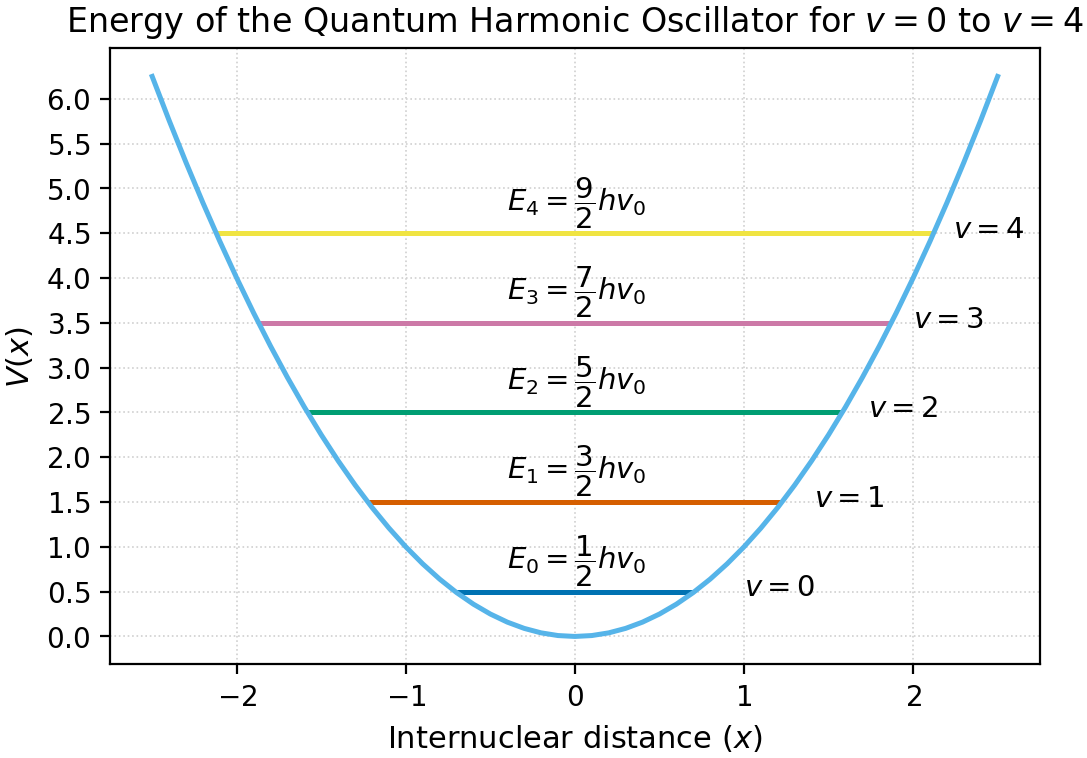
\includegraphics[width=0.7\linewidth]{Energy_levels}
  \caption{Schematic energy level diagram.}
  \label{fig:levels}
\end{figure}

Figure~\ref{fig:levels} shows a typical structure that recurs
throughout the rest of these notes. A few fundamental constants
are collected in Table~\ref{tab:constants} for reference.

\begin{table}[ht]
  \centering
  \caption{Fundamental physical constants.}
  \label{tab:constants}
  \begin{tabular}{lcr}
    \toprule
    Quantity            & Symbol  & Value                         \\
    \midrule
    Speed of light      & $c$     & $2.998 \times 10^8$ m/s       \\
    Planck's constant   & $\hbar$ & $1.055 \times 10^{-34}$ Js    \\
    Elementary charge   & $e$     & $1.602 \times 10^{-19}$ C     \\
    \bottomrule
  \end{tabular}
\end{table}


% ============================================================
\section{Numerical Methods}

% TikZ figure example: use darkorange for energy levels / structural
% elements, darkolive for curves / wave functions, black for axes and
% walls, and gray for secondary labels.  darkred is reserved for
% hyperlinks and the separator rule -- do not use it in figures.
\begin{figure}[H]
  \centering
  \begin{tikzpicture}[>=stealth]
    % Potential well walls and floor
    \draw[very thick] (0,0) -- (0,4);
    \draw[very thick] (4,0) -- (4,4);
    \draw[thick]      (-0.3,0) -- (4.3,0);
    % Energy axis
    \draw[->,thick] (-0.8,0) -- (-0.8,4.2)
      node[above,font=\small] {$E$};
    % Energy levels (darkorange)
    \foreach \n/\y in {1/0.65, 2/1.70, 3/3.10} {
      \draw[darkorange,thick] (0,\y) -- (4,\y);
      \node[right,font=\small,darkorange] at (4.15,\y) {$E_{\n}$};
    }
    % Wave functions (darkolive), one half-period per quantum number
    \draw[darkolive,thick,domain=0:4,samples=80]
      plot (\x, {0.65 + 0.38*sin(deg(\x*3.14159/4))});
    \draw[darkolive,thick,domain=0:4,samples=80]
      plot (\x, {1.70 + 0.38*sin(deg(2*\x*3.14159/4))});
    \draw[darkolive,thick,domain=0:4,samples=80]
      plot (\x, {3.10 + 0.38*sin(deg(3*\x*3.14159/4))});
    % x-axis labels (gray for secondary info)
    \node[below,font=\small,gray] at (0,-0.1) {$0$};
    \node[below,font=\small,gray] at (4,-0.1) {$L$};
  \end{tikzpicture}
  \caption{Infinite square well: energy levels $E_n \propto n^2$
           (\textcolor{darkorange}{orange}) and corresponding
           eigenfunctions $\psi_n$ (\textcolor{darkolive}{olive}).}
  \label{fig:well}
\end{figure}

The \verb|python| environment typesets code with Gruvbox Light
syntax highlighting directly in the notes — well suited for short
scripts that accompany an analytical derivation. The running example
is the infinite square well, shown in Figure~\ref{fig:well} with its
first three energy levels and eigenfunctions.

The script below evaluates the probability density
$|\psi_n(x)|^2$ numerically,
then integrates $\langle x \rangle = \int_0^L x\,|\psi_n|^2\,\mathrm{d}x$
for the first three levels and confirms the result $\langle x \rangle = L/2$.

\begin{python}
import numpy as np

def psi(n, x, L=1.0):
    """Normalized wavefunction for the infinite square well."""
    return np.sqrt(2.0 / L) * np.sin(n * np.pi * x / L)

def energy(n, L=1.0, hbar=1.0, m=1.0):
    """Energy eigenvalue E_n in natural units."""
    return (n * np.pi * hbar)**2 / (2 * m * L**2)

x = np.linspace(0, 1, 1000)
for n in range(1, 4):
    prob = psi(n, x)**2          # probability density |psi_n|^2
    mean_x = np.trapz(x * prob, x)
    print(f"n={n}  E_n={energy(n):.4f}  <x>={mean_x:.4f}")
\end{python}

Running this prints $\langle x \rangle \approx 0.5000$ for all~$n$,
consistent with the symmetry of each eigenstate about the midpoint
of the well.


% ============================================================
\section{Exercises}

Notes can carry problems alongside the exposition. The
\verb|exercise| environment is numbered per section and is
visually separated from the surrounding text by
\verb|\separator|. Subproblems use the \verb|subproblems|
environment, which labels parts a), b), c) without affecting
ordinary \verb|enumerate| lists.

\separator

\begin{exercise}[Eigenvalues and orthogonality]
  Show that the eigenvalues of a self-adjoint operator
  $\hat{A}$ are real, and that eigenvectors belonging to
  distinct eigenvalues are orthogonal.
\end{exercise}

\begin{exercise}[Infinite square well]
  Consider a particle in a one-dimensional infinite square
  well of width $L$.
  \begin{subproblems}
    \item Write down the normalized energy eigenfunctions.
    \item Compute the energy levels $E_n$.
  \end{subproblems}

  The remaining parts build on the spectrum found above; use
  the result from part~(b) when sketching the densities.

  \begin{subproblems}[resume]
    \item Sketch the probability density for $n = 1, 2, 3$.
    \item Compute the expectation value $\langle x \rangle$ in
          the ground state.
  \end{subproblems}
\end{exercise}


% ============================================================
\section{Closing}

These notes are a template; the content above exists only to
demonstrate typography. Replace it with your own material as the
notes develop.


% ============================================================
% BIBLIOGRAPHY
% ============================================================
\bibliographystyle{unsrtnat}
\bibliography{references}


\end{document}
